\documentclass[11pt]{exam}
\usepackage[utf8]{inputenc}
\usepackage[spanish,activeacute]{babel}
\usepackage{siunitx}
\pagestyle{empty}
\usepackage{wrapfig}
\usepackage{amssymb}
\usepackage{comment}
\usepackage{amsmath}
\usepackage{graphicx}
\usepackage{upgreek} % para poner letras griegas sin cursiva
\usepackage{cancel} % para tachar
\usepackage{mathdots} % para el comando \iddots
\usepackage{mathrsfs} % para formato de letra
\usepackage{stackrel} % para el comando \stackbin
\usepackage{pstricks}
\usepackage{marginnote}
\usepackage{tcolorbox}
\tcbuselibrary{theorems}


\usepackage[paperheight=13in,paperwidth=8.5in,margin=0.5in]{geometry}
\firstpageheadrule
\firstpageheader{Física I - Modular}{}{Universidad del Bío-Bío }
\runningfooter{}{}{}

%cambiar palabras a español
\pointpoints{punto}{puntos}
\hpword{Puntos:}
\vpword{Puntaje}
\htword{Total}
\vtword{Total:}
\vsword{Obtenido}

% ESPACIOS
%\vspace*{60pt}
%\vspace*{\stretch{1}}

\begin{document}


\pointname{}
\boxedpoints
\begin{comment}
\begin{center}
 \includegraphics[width=1cm]{figs/logoubb.png}\\
\Large{\textbf{ Certamen 2 }}\\
Física I Módulo 2 - Fase 2 - Ingenierias en Construcción  S1-2020\\
\end{center}
\bigskip

\hbox to \textwidth{\enspace\hrulefill}
\hspace*{\stretch{1}} Apellido Paterno \hspace*{\stretch{1}} Apellido Materno  \hspace*{\stretch{1}} Nombres \hspace*{\stretch{1}}\\
\\
\\
\\
%\begin{table}[htbp]
%\begin{center}
%\begin{tabular}{||c|c|c|c|}
%\hline
%Profesor   & P. Flores  & E. Riveros \\
%\hline \hline
%Marcar X &   &  \\
%                  & &\\ \hline
%\end{tabular}
%\caption{Profesor}
%\label{tabla:sencilla}
%\end{center}
%\end{table}




\bigskip
\vqword{Problema}
\addpoints
\vspace*{\stretch{1}}
\begin{center}
	\Large
	\gradetable  %TABLA DE PUNTAJES
\end{center}
\vspace*{\stretch{2}}
\newpage
\end{comment}

\begin{questions}
	



%%%%%%%%%% PROBLEMA 1 ---- EQUILIBRIO -----%%%%%%%%%%%%%%%%%%%%%%%%%
%%%%%%%%%%%%%%%% PAUTA %%%%%%%%%%%%
%\begin{questions} 

\begin{minipage}[c]{11cm}
 \question[19] Considere un solenoide de radio $r=5[cm]$ con $n=400$ [vueltas/metro] por el que circula una corriente dada por $I(t)=3e^{3t}[A]$. Fuera del solenoide, pero concentrico a él, se encuentra una bobina de radio $R=2r$ con $N=20$ espiras, la que también tiene conectada una resistencia de $R=20\Omega$. En las figuras adjuntas, se muestran las vistas aéreas y de corte longitudinal del sistema. Calcule:\\
  
  \end{minipage}
 \begin{minipage}[c]{5cm}
 \hspace{0,5cm}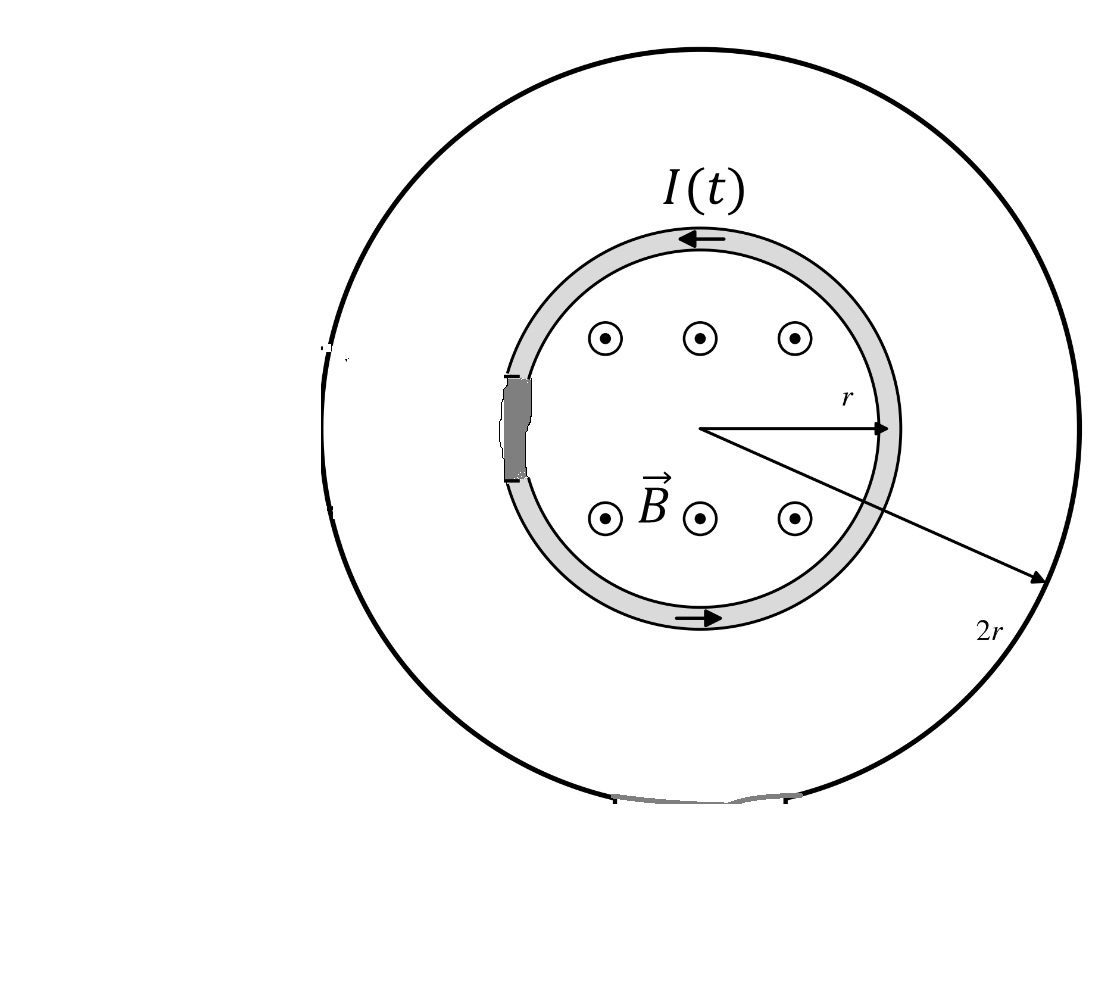
\includegraphics[scale=0.15]{bobinas-vista-aerea.jpg}
 %\end{minipage}
 %\begin{minipage}[c]{5cm}
 \hspace{0,5cm}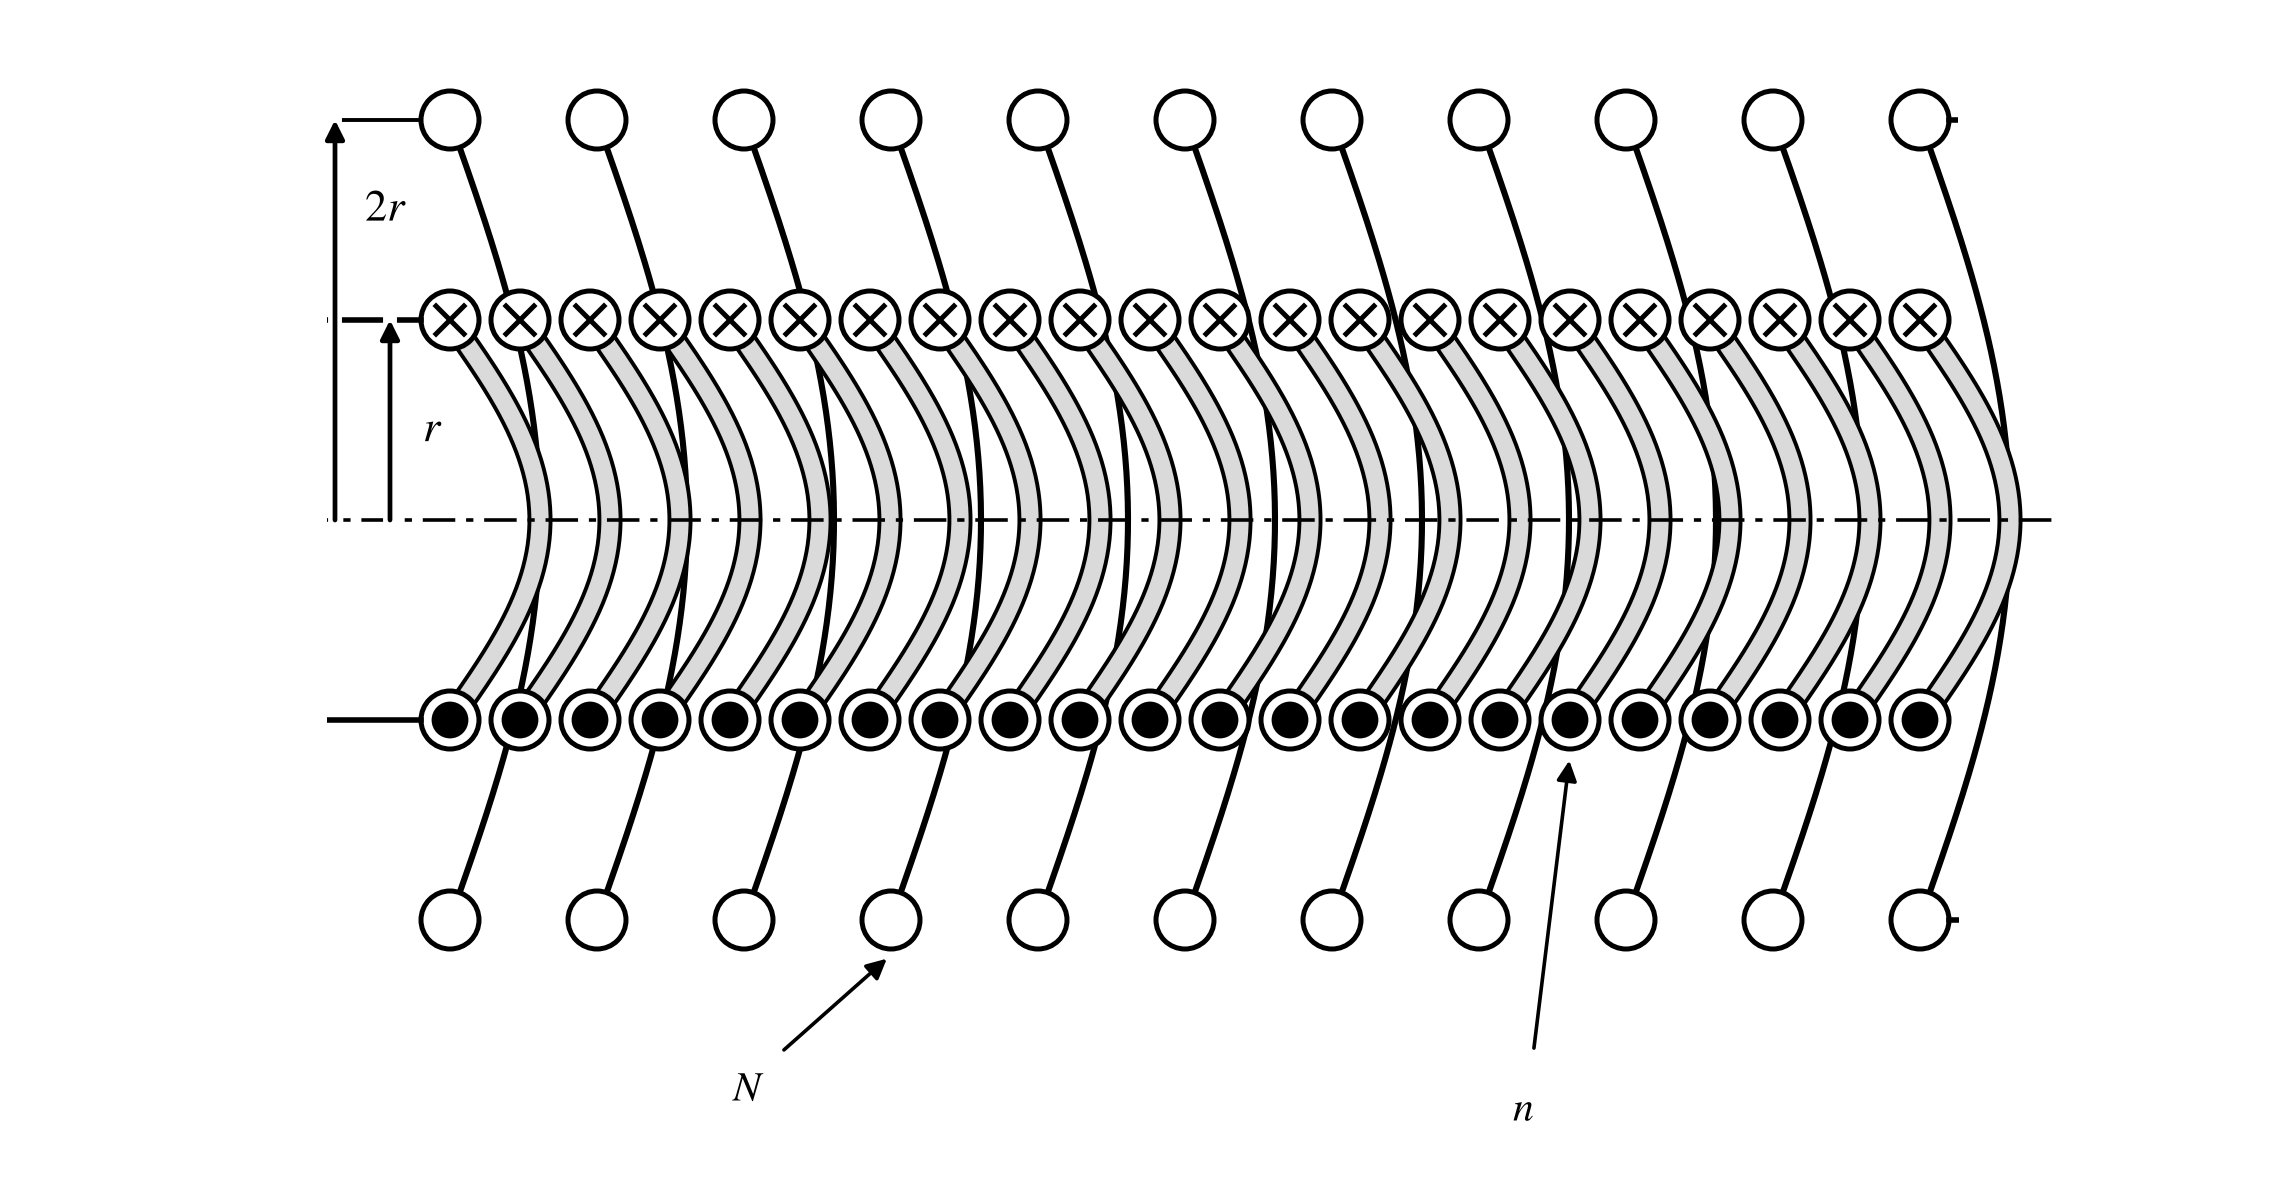
\includegraphics[scale=0.20]{corte_longitudinal_bobinas_bn.png}
  \end{minipage}
  \\
  (a)\textbf{(7.0 pts)}El flujo magnético $\Phi_B$ a través de la bobina. \\
  \vspace{10cm}
\begin{comment}
\begin{minipage}{0.3\textwidth}
\centering
\includegraphics[scale=0.30]{figs/DCL-barra.png}\\
{\bf\red(4.0 pts)}
\end{minipage}
\begin{minipage}{0.3\textwidth}
\centering
\includegraphics[scale=0.30]{figs/DCL-masa2.png}\\
{\bf\red(2.0 pts)}
\end{minipage}
\begin{minipage}{0.3\textwidth}
\centering
\includegraphics[scale=0.30]{figs/DCL-nodo.png}\\
{\bf\red(3.0 pts)}
\end{minipage}\\
\end{comment}

(b)\textbf{(6.0 pts)} La fem inducida.\\
\vspace{6cm}

(c)\textbf{(6.0 pts)} La corriente inducida, determine. de acuerdo a la ley de Lenz el sentido del campo magnético inducido.\\
\vspace{4cm}

\begin{comment}
 \begin{align}
  {\hbox De la ecuación (7) en (9) obtenemos:}\nonumber\\
  T_3&=\frac{T_2}{\sin 53^0} = 87,6[N] \ \ \ {\bf\red(2.0 pts)}\\
  {\hbox Reemplazamos en la ecuación (8)}\nonumber\\
  T_1&= 52,7[N] \ \ \ {\bf\red(1.0 pts)} \nonumber\\
 {\hbox Luego en la ecuación (6)} \nonumber\\
 \hat{k}&:\ \ \ -20m_1 -80 + 8T_1 = 0 \implies m_1=\frac{80 - 8T_1}{-20}\\
 M_1=17,1[kg] \ \ \ {\bf\red(3.0 pts)}
 \end{align}
\end{comment}

%\end{comment}
%\newpage
%---------------------------------------------------------------------
%_______________ PROBLEMA 2________________________________________
%------------------------------------------------------- 
 \newpage
 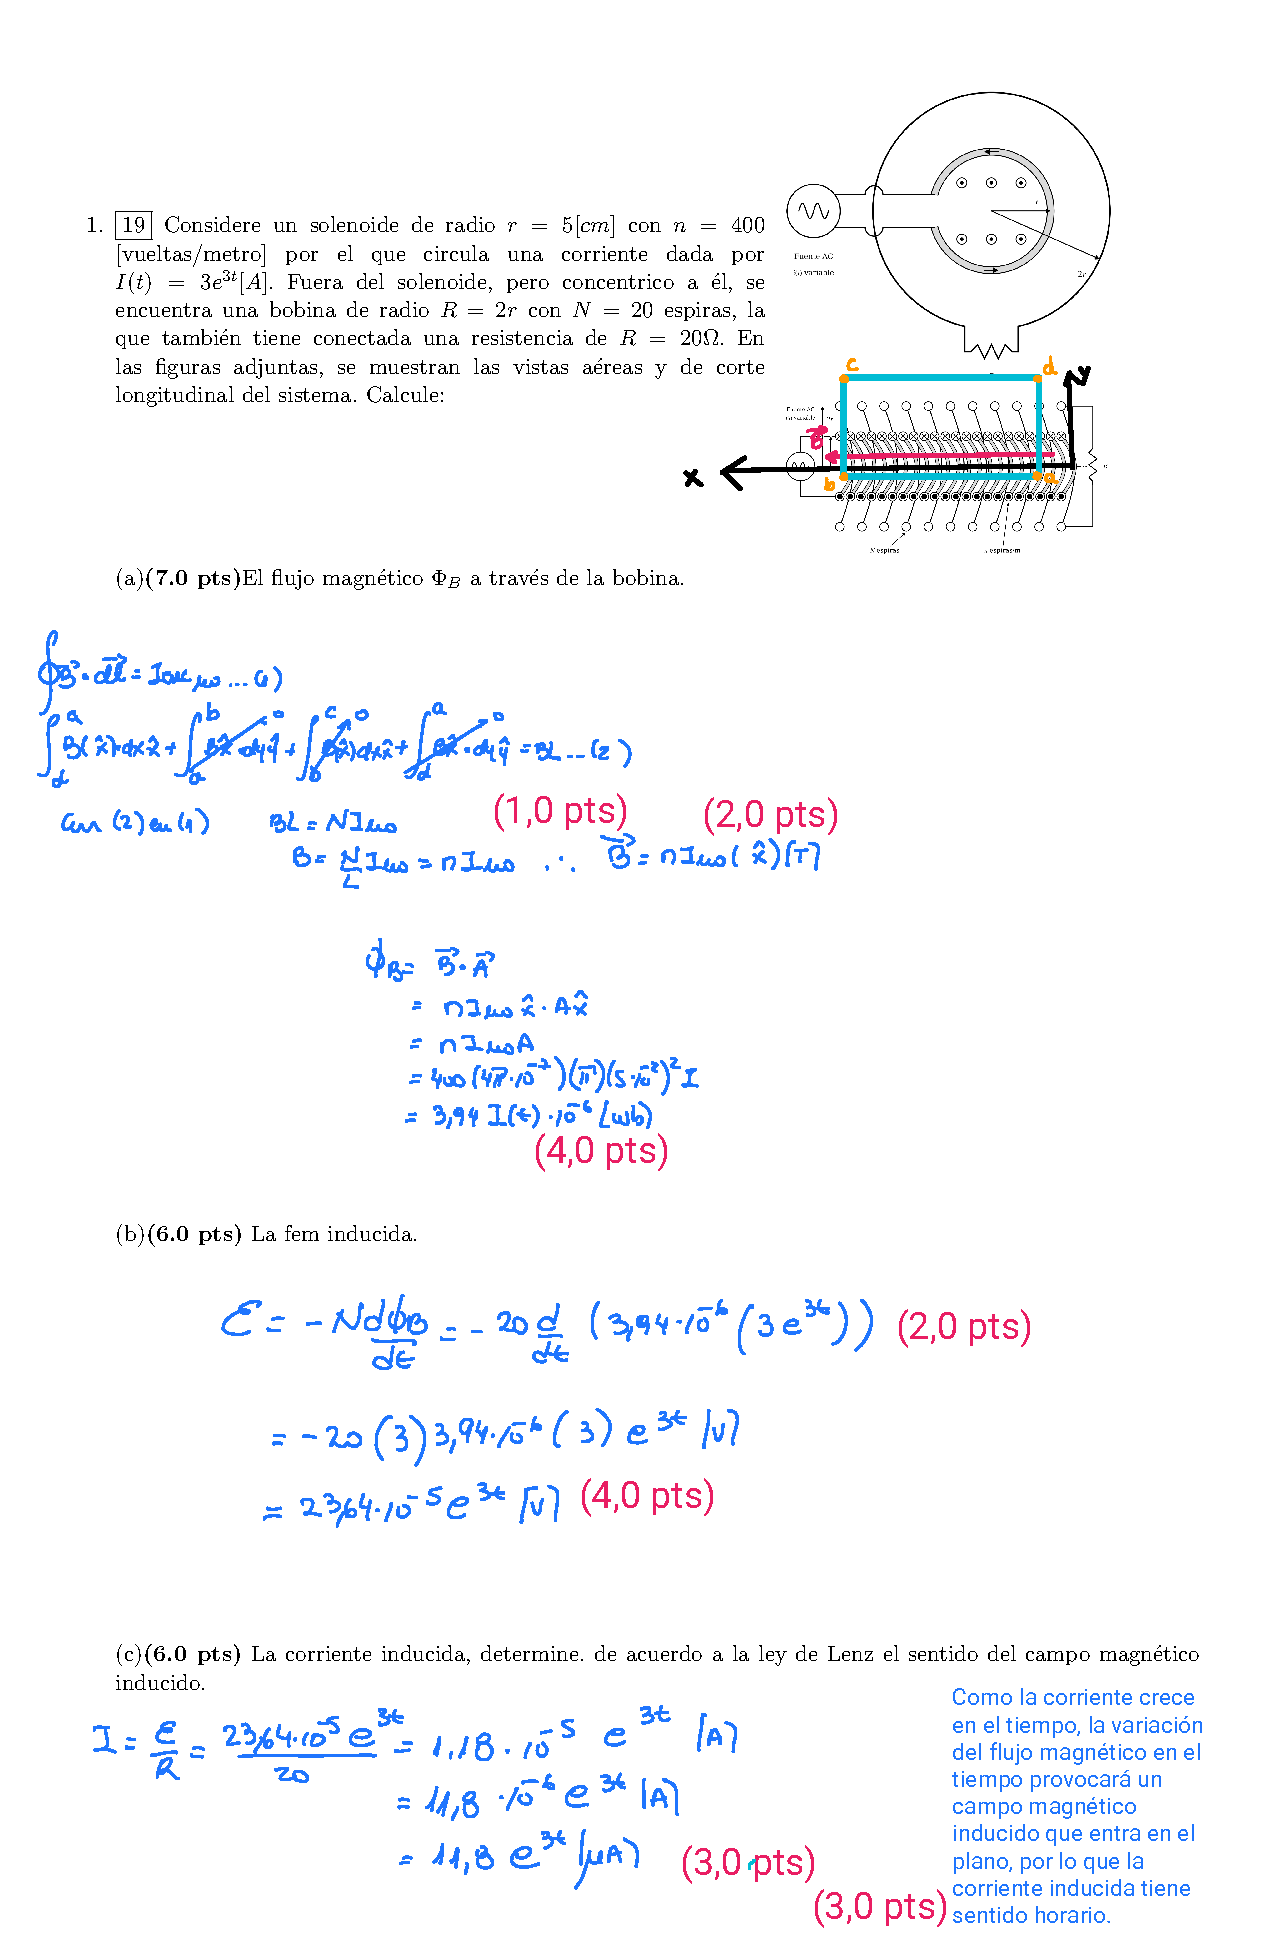
\includegraphics[scale=0.9]{P3_VB_C4_electro_S2_2026_PAUTA (1) (1).pdf}
 \begin{comment}
     
 
\begin{minipage}[c]{10cm}
 \question[19] Considere un solenoide de radio $r=5[cm]$ con $n=400$ [vueltas/metro] por el que circula una corriente dada por $I(t)=\frac{1}{6}e^{-3t}[A]$. Fuera del solenoide, pero concentrico a él, se encuentra una bobina de radio $R=2r$ con $N=20$ espiras, la que también tiene conectada una resistencia de $R=20\Omega$. Calcule:\\\\
  
  \end{minipage}
 \begin{minipage}[c]{9cm}
 \hspace{0,5cm}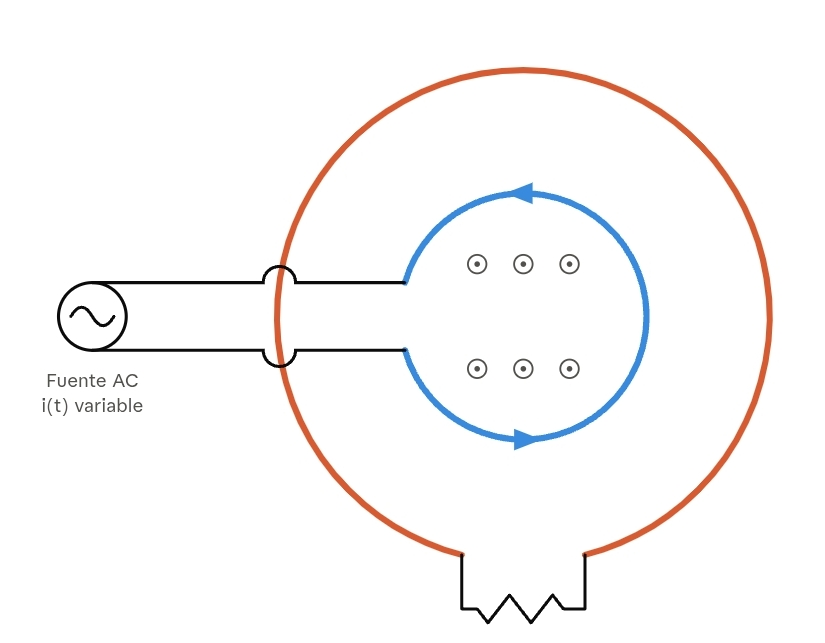
\includegraphics[scale=0.30]{bobinas.jpg}
  \end{minipage}
    (a)\textbf{(7.0 pts)}El flujo magnético $\Phi_B$ a través de la bobina. \\
  \vspace{10cm}\\


(b)\textbf{(6.0 pts)} La fem inducida.\\
\vspace{5cm}\\

(c)\textbf{(6.0 pts)} La corriente inducida, determine. de acuerdo a la ley de Lenz el sentido del campo magnético inducido.\\
\end{comment}
   \end{questions} 
\end{document}
